
\documentclass{beamer}
\usecolortheme{dove}
\setbeamertemplate{navigation symbols}{}
\usepackage{amsmath,amssymb,amsfonts,amsthm, multicol, subfigure, color}
\usepackage{bm}
\usepackage{graphicx}
\usepackage{tabularx}
\usepackage{booktabs}
\usepackage{hyperref}
\usepackage{pdfpages}
\usepackage{xcolor}
\definecolor{seagreen}{RGB}{46, 139, 87}
\def\independenT#1#2{\mathrel{\rlap{$#1#2$}\mkern2mu{#1#2}}}
\newcommand\indep{\protect\mathpalette{\protect\independenT}{\perp}}
\def\log{\text{log}}
\newcommand\logit{\text{logit}}
\newcommand\iid{\stackrel{\text{iid}}{\sim}}
\newcommand\E{\text{E}}
\newcommand\V{\text{V}}
\renewcommand\P{\text{P}}
\newcommand{\Cov}{\text{Cov}}
\newcommand{\Cor}{\text{Cor}}
\newcommand\doop{\text{do}}
\usepackage{stackrel}
\usepackage{tikz}
\usetikzlibrary{arrows,shapes.arrows,positioning,shapes,patterns,calc}
\newcommand\slideref[1]{\vskip .1cm \tiny \textcolor{gray}{{#1}}}
\newcommand\red[1]{\color{red}#1}
\newcommand\blue[1]{\color{blue}#1}
\newcommand\gray[1]{\color{gray}#1}
\newcommand\seagreen[1]{\color{seagreen}#1}
\newcommand\purple[1]{\color{purple}#1}
\newcommand\orange[1]{\color{orange}#1}
\newcommand\black[1]{\color{black}#1}
\newcommand\white[1]{\color{white}#1}
\newcommand\teal[1]{\color{teal}#1}
\newcommand\magenta[1]{\color{magenta}#1}
\newcommand\Fuchsia[1]{\color{Fuchsia}#1}
\newcommand\BlueGreen[1]{\color{BlueGreen}#1}
\newcommand\bblue[1]{\textcolor{blue}{\textbf{#1}}}
\newcommand\bred[1]{\textcolor{red}{\textbf{#1}}}
\newcommand\bgray[1]{\textcolor{gray}{\textbf{#1}}}
\newcommand\bgreen[1]{\textcolor{seagreen}{\textbf{#1}}}
\newcommand\bref[2]{\href{#1}{\color{blue}{#2}}}
\colorlet{lightgray}{gray!40}
\pgfdeclarelayer{bg}    % declare background layer for tikz
\pgfsetlayers{bg,main} % order layers for tikz
\newcommand\mycite[1]{\begin{scriptsize}\textcolor{darkgray}{(#1)}\end{scriptsize}}
\newcommand{\tcframe}{\frame{
%\small{
\only<1|handout:0>{\tableofcontents}
\only<2|handout:1>{\tableofcontents[currentsubsection]}}
%}
}

\usepackage[round]{natbib}
\bibliographystyle{humannat-mod}
\setbeamertemplate{enumerate items}[default]
\usepackage{mathtools}

\newcommand{\goalsframe}{\begin{frame}{Learning goals for today}
\begin{itemize}
    \item fundamental problem of causal inference
    \item potential outcomes
    \item recall mathematical concepts from probability
    \begin{itemize}
    \item random variables
    \item expectation
    \item conditional expectation
    \end{itemize}
\end{itemize} \vskip .2in
\end{frame}}

\title{Causal Inference: Potential Outcomes}
\author{Ian Lundberg\footnote{Assistant Professor, Information Science, Cornell, \href{mailto:ilundberg@cornell.edu}{ilundberg@cornell.edu}} \& Kristin Liao\footnote{PhD Student, Sociology, UCLA, \href{mailto:ktliao@g.ucla.edu}{ktliao@g.ucla.edu}}}
\date{SICSS UCLA\\24 June 2024}

\begin{document}

\maketitle

\goalsframe

\begin{frame}{Causal claims hinge on arguments, not on data}

\includegraphics[width = .6\textwidth]{figures/Biles_bar}
\includegraphics[width = .3\textwidth]{figures/Biles_medal}

\vskip .2in
\begin{tiny}
Left photo: By Fernando Frazão/Agência Brasil - \url{http://agenciabrasil.ebc.com.br/sites/_agenciabrasil2013/files/fotos/1035034-_mg_0802_04.08.16.jpg, CC BY 3.0 br, https://commons.wikimedia.org/w/index.php?curid=50548410} \\
Right photo: By Agencia Brasil Fotografias - EUA levam ouro na ginástica artística feminina; Brasil fica em 8 lugar, CC BY 2.0, \url{https://commons.wikimedia.org/w/index.php?curid=50584648}\\
\end{tiny}

\end{frame}

\begin{frame}{Causal claims hinge on arguments, not on data}
\begin{enumerate}
\item Statistical evidence
\begin{itemize}
\item Simone Biles swung on the uneven bars. She won a gold medal. \pause
\item I did not swing on the uneven bars. I did not win a gold medal.
\end{itemize} \pause
\item Possible causal claim
\begin{itemize}
\item Swinging on the uneven bars causes a person to win a gold medal.
\end{itemize}
\end{enumerate} \vskip .2in \pause
\begin{tabular}{rccc}
& \multicolumn{2}{l}{Do you win gold if you:} & Causal effect \\
& Swing & Do not swing & of swinging \\
\hline
Simone Biles & Yes (1) & \only<1-4>{?}\only<5->{\blue{No (0)}} & \only<1-5>{?}\only<6->{+1} \\
Ian & \only<1-6>{?}\only<7->{\blue{No (0)}} & No (0) & \only<1-7>{?}\only<8->{0} \\
\hline
\end{tabular}
\end{frame}

\begin{frame}
\includegraphics[width = \textwidth]{figures/mediterranean_diet}
\end{frame}

\begin{frame}{Fundamental problem of causal inference}{\href{https://www.tandfonline.com/doi/abs/10.1080/01621459.1986.10478354}{Holland 1986}}

\begin{tikzpicture}[x = \textwidth, y = .8\textheight]
\node at (0,0) {};
\node at (1,1) {};
% Factual outcomes
\node[anchor = north, align = center] at (.25,1) {Descriptive evidence};
\foreach \i in {1,...,8} {
	\node[font = \tiny, anchor = west] at (-.05,9/20-\i/20 + .175) {Person \i};
}
\foreach \i in {.2,.3,.35,.45,.55} {
	\draw[fill = blue, opacity = .3, color = blue] (.05,\i) rectangle (.25,\i + .05) {};
	\node[font = \tiny] at (.15,\i + .025) {lifespan};
}
\foreach \i in {.25,.4,.5} {
	\draw[fill = seagreen, opacity = .3, color = seagreen] (.25,\i) rectangle (.45,\i + .05) {};
	\node[font = \tiny] at (.35,\i + .025) {lifespan};
}
\node[font = \footnotesize, align = center, fill = blue, fill opacity = .3, text opacity = 1] at (.15,.8) {average\\lifespan};
\node[font = \footnotesize, align = center, fill = seagreen, fill opacity = .3, text opacity = 1] at (.35,.8) {average\\lifespan};
\node at (.25,.8) {$-$};
%\node[font = \tiny] at (.15,.575) {$Y_1^\text{Mediterranean Diet}$};
%\node[font = \tiny] at (.35,.525) {$Y_2^\text{Standard Diet}$};
%\node[font = \tiny] at (.15,.475) {$Y_3^\text{Mediterranean Diet}$};
%\node[font = \tiny] at (.35,.425) {$Y_4^\text{Standard Diet}$};
%\node[font = \tiny] at (.15,.375) {$Y_5^\text{Mediterranean Diet}$};
%\node[font = \tiny] at (.15,.325) {$Y_6^\text{Mediterranean Diet}$};
%\node[font = \tiny] at (.35,.275) {$Y_7^\text{Standard Diet}$};
%\node[font = \tiny] at (.15,.225) {$Y_8^\text{Mediterranean Diet}$};
\node[anchor = north, align = center, font = \footnotesize, blue] at (.15, .2) {Outcome\\under\\Mediterranean\\diet};
\node[anchor = north, align = center, font = \footnotesize, seagreen] at (.35, .2) {Outcome\\under\\standard\\diet};
\pause
% Potential outcomes
\node[anchor = north, align = center] at (.75,1) {Causal claim};
\node[font = \footnotesize, align = center, fill = blue, fill opacity = .3, text opacity = 1] at (.65,.8) {average\\lifespan};
\node[font = \footnotesize, align = center, fill = seagreen, fill opacity = .3, text opacity = 1] at (.85,.8) {average\\lifespan};
\node at (.75,.8) {$-$};
\foreach \i in {.2,.25,.3,.35,.4,.45,.5,.55} {
	\draw[fill = blue, opacity = .3, color = blue] (.55,\i) rectangle (.75,\i + .05) {};
	\draw[fill = seagreen, opacity = .3, color = seagreen] (.75,\i) rectangle (.95,\i + .05) {};
	\node[font = \tiny] at (.65,\i + .025) {lifespan};
	\node[font = \tiny] at (.85,\i + .025) {lifespan};
}
\node[anchor = north, align = center, font = \footnotesize, blue] at (.65, .2) {Outcome\\under\\Mediterranean\\diet};
\node[anchor = north, align = center, font = \footnotesize, seagreen] at (.85, .2) {Outcome\\under\\standard\\diet};
\pause
\foreach \i in {.2,.3,.35,.45,.55} {
	\node[font = \tiny, red] at (.35,\i + .025) {missing};
}
\foreach \i in {.25,.4,.5} {
	\node[font = \tiny, red] at (.15,\i + .025) {missing};
}
\pause
\node at (.5,.66) {Causal inference is a \bred{missing data} problem};
\end{tikzpicture}
\end{frame}

\begin{frame}{Mathematical notation: Potential outcomes} \pause

\begin{tabular}{lll}
$Y_i$ & Outcome & Whether person $i$ survived \\ \pause
$A_i$ & Treatment & Whether person $i$ ate a Mediterranean diet \\ \pause
$Y_i^a$ & Potential Outcome & Outcome person $i$ would realize if \\&&assigned to treatment value $a$ \pause
\end{tabular} \vskip .2in
Examples:
\begin{footnotesize}
\begin{align*}
\onslide<5->{Y_\text{Ian} &= \texttt{survived} && \text{Ian survived} \\}
\onslide<6->{A_\text{Ian} &= \texttt{MediterraneanDiet} && \text{Ian ate a Mediterranean diet} \\}
\onslide<7->{Y_\text{Ian}^\text{MediterraneanDiet} &= \texttt{survived} && \text{Ian would survive on a Mediterranean diet} \\}
\onslide<8->{Y_\text{Ian}^\text{StandardDiet} &= \texttt{died} && \text{Ian would die on a standard diet}}
\end{align*} \vskip .1in
\end{footnotesize}
\onslide<9->{\bgray{Discuss.}\\Which potential outcome is observed?\\Which is counterfactual?}

\end{frame}

\begin{frame}{The consistency assumption}
\begin{tikzpicture}[x = \textwidth, y = .8\textheight]
\onslide<2->{
\draw[thick] (0,.6) -- (.4, .6) -- (.4,0);
\node[anchor = south] at (.2,0) {Potential Outcomes};
\node at (.15,.4) {$Y_i^\text{MediterraneanDiet}$};
\node at (.25,.25) {$Y_i^\text{StandardDiet}$};
}
\onslide<3->{\draw[thick] (1,.6) -- (.6, .6) -- (.6,0);
\node[anchor = south] at (.8,0) {Factual Outcomes};
\node at (.8,.35) {$Y_i$};
}
\onslide<4->{
\node[anchor = south, align = center, blue, draw, rounded corners, line width = 1.2pt, inner sep = 12pt] at (.5,.65) {Consistency Assumption\\$Y_i^{A_i} = Y_i$};
}
\end{tikzpicture}
\end{frame}

\begin{frame}{Mathematical notation: Potential outcomes are fixed}
A person's potential outcome is a \bblue{fixed quantity} \pause
$$Y_\text{Ian}^\text{MediterraneanDiet}=\texttt{survived}$$
\vskip .2in \pause
The outcome for a random person is a \bblue{random variable} \pause
\begin{itemize}
\item Draw a random person from the population \pause
\item Assign them a Mediterranean diet \pause
\item The outcome $Y^\text{MediterraneanDiet}$ is a random variable:
\begin{itemize}
\item takes the value \texttt{survived} if we randomly sample some people
\item takes the value \texttt{died} if we randomly sample others
\end{itemize}
\end{itemize} \pause
\bgray{Check for understanding:}\\Does it make sense to write $\V(Y_i^a)$? How about $\V(Y^a)$

\end{frame}

\begin{frame}{Notation: Expectation operator}
The \bblue{expectation operator} $\E()$ denotes the population mean
$$\E(Y^a) = \frac{1}{n}\sum_{i=1}^n Y_i^a$$
The quantity $Y^a$ inside the expectation must be a random variable \pause \vskip .6in
A \bblue{conditional expectation} is denoted with a vertical bar
$$\E(Y\mid A = a) = \frac{1}{n_a}\sum_{i:A_i=a} Y_i$$
\end{frame}

\subsection{Practicing notation}

\begin{frame}{Practice: How would you say this in English?}
We might wonder how a person's earnings relate to whether they hold a college degree \vskip .2in
\begin{enumerate}
\item $\E(\text{Earnings} \mid \text{Degree} = \texttt{TRUE}) > \E(\text{Earnings} \mid \text{Degree} = \texttt{FALSE})$
\onslide<2->{\begin{itemize}
\item Average earnings are higher among those with college degrees
\end{itemize}}\vskip .4in
\item $\E(\text{Earnings}^{\text{Degree} = \texttt{TRUE}}) > \E(\text{Earnings}^{\text{Degree} = \texttt{FALSE}})$ \vskip .1in
\onslide<3->{\begin{itemize}
\item On average, a degree causes higher earnings
\end{itemize}
}
\end{enumerate}
\end{frame}

\begin{frame}{Practice: How would you write this in math?}

\begin{enumerate}
\item On average, students who do the homework learn more than those who don't
\onslide<2->{$$\E(\text{Learning}\mid \text{HW} = \texttt{TRUE}) > \E(\text{Learning}\mid \text{HW} = \texttt{FALSE})$$}
\item On average, doing the homework causes more learning
\onslide<3->{$$\E(\text{Learning}^{\text{HW} = \texttt{TRUE}}) > \E(\text{Learning}^{\text{HW} = \texttt{FALSE}})$$}
\end{enumerate}

\end{frame}

\goalsframe

\begin{frame}{Resources to learn more}
\begin{itemize}
\item Hernán, M.A., \& J.M. Robins. 2020.\\\bref{https://www.hsph.harvard.edu/miguel-hernan/causal-inference-book/}{Causal Inference: What If?}\\Boca Raton: Chapman \& Hall / CRC.
\item Imbens, G. W., \& Rubin, D. B. 2015.\\\bref{https://www.cambridge.org/core/books/causal-inference-for-statistics-social-and-biomedical-sciences/71126BE90C58F1A431FE9B2DD07938AB}{Causal Inference in Statistics, Social, and Biomedical Sciences.}\\Cambridge University Press.
\item Brand, J. E. 2023.\\\bref{https://www.russellsage.org/publications/overcoming-odds}{Overcoming the Odds: The Benefits of Completing College for Unlikely Graduates.}\\Russell Sage Foundation.
\end{itemize}
\end{frame}

\end{document}
